%==============================================================
%  Figura 6.12 - Graduazione dei requisiti per il software
%  correlato alla sicurezza (EN ISO 13849-1)
%  Adattamento in italiano della Figura 6.12 dell'IFA Report 2/2017
%
%  Le coordinate sono state ricavate dalla grafica vettoriale
%  dell'originale (pagina 68 di rep0217e.pdf) e sono espresse nei
%  punti PostScript di quel disegno; l'unita' della tikzpicture
%  (x=y=0.042cm) riporta il tutto alle proporzioni originali.
%
%  Sistema di riferimento: l'origine e' l'angolo in basso a sinistra
%  della cornice esterna; l'asse y e' rivolto verso l'alto.
%
%  I riquadri interni hanno il bordo inferiore "strappato": una curva
%  di Bezier a S con i due punti di controllo sulla verticale mediana
%  del riquadro, come nell'originale. Il bordo scende sotto la fascia
%  grigia che li contiene, quindi vanno disegnati dopo di essa.
%
%  Il corpo e' \footnotesize: le diciture italiane sono piu' lunghe
%  delle inglesi e "Riferimento:" non entrerebbe nel riquadro piu'
%  stretto, che qui ha le dimensioni dell'originale.
%==============================================================
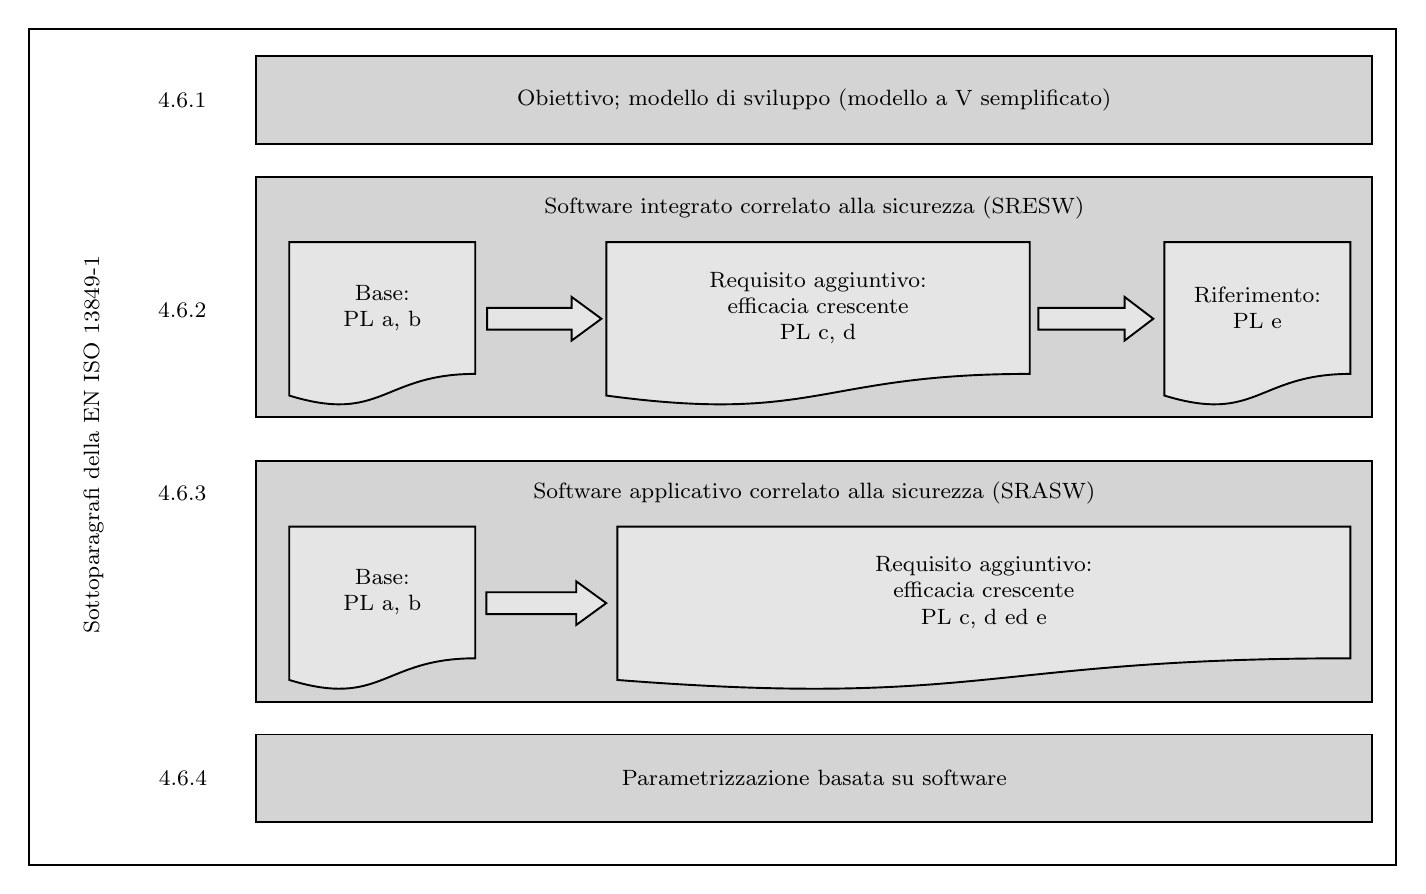
\begin{tikzpicture}[
  x=0.042cm, y=0.042cm,
  font=\footnotesize,
  cornice/.style={draw=black, line width=0.9pt},
  fascia/.style={draw=black, fill=black!17, line width=0.69pt},
  strappato/.style={draw=black, fill=black!10, line width=0.69pt},
  frecciona/.style={draw=black, fill=black!10, line width=0.69pt}
]

\setstretch{1}

% --- 4.6.1 ----------------------------------------------------------------
\draw[fascia] (69.10,218.40) rectangle (406.53,244.87);
\node at (46.76,231.64) {4.6.1};
\node at (237.82,231.64) {Obiettivo; modello di sviluppo (modello a V semplificato)};

% --- 4.6.2: software integrato (SRESW) ------------------------------------
\draw[fascia] (69.10,135.70) rectangle (406.53,208.48);
\node at (46.76,167.95) {4.6.2};
\node at (237.82,198.85) {Software integrato correlato alla sicurezza (SRESW)};

\draw[strappato] (79.09,188.65) -- (135.32,188.65) -- (135.32,148.82)
  .. controls (107.20,148.82) and (107.20,133.65) .. (79.09,142.27) -- cycle;
\node[align=center] at (107.21,168.70) {Base:\\PL a, b};

\draw[strappato] (174.96,188.65) -- (302.97,188.65) -- (302.97,148.82)
  .. controls (238.97,148.82) and (238.97,133.65) .. (174.96,142.27) -- cycle;
\node[align=center] at (238.97,168.70)
  {Requisito aggiuntivo:\\efficacia crescente\\PL c, d};

\draw[strappato] (343.67,188.65) -- (399.90,188.65) -- (399.90,148.82)
  .. controls (371.79,148.82) and (371.79,133.65) .. (343.67,142.27) -- cycle;
\node[align=center] at (371.79,168.70) {Riferimento:\\PL e};

\draw[frecciona] (138.92,168.79) -- (164.46,168.79) -- (164.46,172.09) --
  (173.46,165.49) -- (164.46,158.89) -- (164.46,162.19) -- (138.92,162.19) -- cycle;
\draw[frecciona] (305.58,168.79) -- (331.63,168.79) -- (331.63,172.09) --
  (340.31,165.49) -- (331.63,158.89) -- (331.63,162.19) -- (305.58,162.19) -- cycle;

% --- 4.6.3: software applicativo (SRASW) ----------------------------------
\draw[fascia] (69.10,49.72) rectangle (406.53,122.50);
\node at (46.76,112.75) {4.6.3};
\node at (237.82,112.75) {Software applicativo correlato alla sicurezza (SRASW)};

\draw[strappato] (79.09,102.67) -- (135.32,102.67) -- (135.32,62.84)
  .. controls (107.20,62.84) and (107.20,47.67) .. (79.09,56.29) -- cycle;
\node[align=center] at (107.21,82.76) {Base:\\PL a, b};

\draw[strappato] (178.27,102.67) -- (399.90,102.67) -- (399.90,62.84)
  .. controls (289.08,62.84) and (289.08,47.67) .. (178.27,56.29) -- cycle;
\node[align=center] at (289.08,82.76)
  {Requisito aggiuntivo:\\efficacia crescente\\PL c, d ed e};

\draw[frecciona] (138.67,82.81) -- (165.85,82.81) -- (165.85,86.11) --
  (174.92,79.52) -- (165.85,72.91) -- (165.85,76.21) -- (138.67,76.21) -- cycle;

% --- 4.6.4 ----------------------------------------------------------------
\draw[fascia] (69.10,13.33) rectangle (406.53,39.80);
\node at (46.96,26.57) {4.6.4};
\node at (237.82,26.57) {Parametrizzazione basata su software};

% --- dicitura verticale a sinistra ----------------------------------------
\node[rotate=90] at (19.96,127.35) {Sottoparagrafi della EN ISO 13849-1};

% --- cornice esterna --------------------------------------------------------
\draw[cornice] (0.38,0.37) rectangle (413.73,253.12);

\end{tikzpicture}
